% Licensed to the Apache Software Foundation (ASF) under one
% or more contributor license agreements.  See the NOTICE file
% distributed with this work for additional information
% regarding copyright ownership.  The ASF licenses this file
% to you under the Apache License, Version 2.0 (the
% "License"); you may not use this file except in compliance
% with the License.  You may obtain a copy of the License at
%
%   http://www.apache.org/licenses/LICENSE-2.0
%
% Unless required by applicable law or agreed to in writing,
% software distributed under the License is distributed on an
% "AS IS" BASIS, WITHOUT WARRANTIES OR CONDITIONS OF ANY
% KIND, either express or implied.  See the License for the
% specific language governing permissions and limitations
% under the License.

\documentclass[twocolumn,9pt]{article}
\usepackage{graphicx}
\usepackage{verbatim}
\oddsidemargin -0.5in
\evensidemargin -0.5in
\textwidth 7.5in
\topmargin -0.75in
\textheight 9in

\begin{document}

\title{Kudu: Storage for Fast Analytics on Fast Data
\footnote{\bf
This document is a draft. Edits will be made and re-published to the Kudu
open source project web site on a rolling basis.}
}
% Authors
%-----------------
\author{
  Todd Lipcon \and David Alves \and Dan Burkert \and Jean-Daniel Cryans \and Adar Dembo \and
  Mike Percy \and Silvius Rus \and Dave Wang \and Matteo Bertozzi \and Colin Patrick McCabe \and
  Andrew Wang\\
  {\small \bf Cloudera, inc.}
}

\date{28 September 2015}

\maketitle

\begin{abstract}
Kudu is an open source storage engine for structured data which supports low-latency random access
together with efficient analytical access patterns. Kudu distributes data using
horizontal partitioning and replicates each partition using Raft consensus, providing low
mean-time-to-recovery and low tail latencies. Kudu is designed within the context of the Hadoop
ecosystem and supports many modes of access via tools such as Cloudera Impala\cite{impala},
Apache Spark\cite{spark}, and MapReduce\cite{mapreduce}.
\end{abstract}

\section{Introduction}
\label{sec:introduction}
In recent years, explosive growth in the amount of data being generated and captured by
enterprises has resulted in the rapid adoption of open source technology which is able to
store massive data sets at scale and at low cost. In particular, the Hadoop ecosystem has become a focal
point for such ``big data'' workloads, because many traditional open source database systems have
lagged in offering a scalable alternative.

Structured storage in the Hadoop ecosystem has typically been achieved in two ways: for static data sets,
data is typically stored on HDFS using binary data formats such as Apache Avro\cite{avro} or
Apache Parquet\cite{parquet}. However, neither HDFS nor these formats has any provision for updating
individual records, or for efficient random access. Mutable data sets are typically stored in
semi-structured stores such as Apache HBase\cite{hbase} or Apache Cassandra\cite{cassandra}. These systems allow for low-latency
record-level reads and writes, but lag far behind the static file formats in terms of sequential
read throughput for applications such as SQL-based analytics or machine learning.

The gap between the analytic performance offered by static data sets on HDFS and the
low-latency row-level random access capabilities of HBase and Cassandra has required
practitioners to develop complex architectures when the need for both access patterns
arises in a single application. In particular, many of Cloudera's customers
have developed data pipelines which involve streaming ingest and updates in HBase, followed
by periodic jobs to export tables to Parquet for later analysis. Such architectures
suffer several downsides:

\begin{enumerate}
\item Application architects must write complex code to manage the
  flow and synchronization of data between the two systems.
\item Operators must manage consistent backups, security policies,
  and monitoring across multiple distinct systems.
\item The resulting architecture may exhibit significant lag between the arrival
  of new data into the HBase ``staging area'' and the time when the new data
  is available for analytics.
\item In the real world, systems often need to accomodate late-arriving data, corrections
  on past records, or privacy-related deletions on data that has already been
  migrated to the immutable store. Achieving this may involve expensive rewriting
  and swapping of partitions and manual intervention.
\end{enumerate}

Kudu is a new storage system designed and implemented from the ground up to fill this gap between
high-throughput sequential-access storage systems such as HDFS\cite{hdfs} and low-latency random-access
systems such as HBase or Cassandra. While these existing systems continue to hold advantages in some
situations, Kudu offers a ``happy medium'' alternative that can dramatically simplify the
architecture of many common workloads. In particular, Kudu offers a simple API for row-level
inserts, updates, and deletes, while providing table scans at throughputs similar to Parquet,
a commonly-used columnar format for static data.

This paper introduces the architecture of Kudu. Section \ref{sec:high-level} describes the system
from a user's point of view, introducing the data model, APIs, and operator-visible constructs.
Section \ref{sec:architecture} describes the architecture of Kudu, including how it partitions and
replicates data across nodes, recovers from faults, and performs common operations.  Section
\ref{sec:storage} explains how Kudu stores its data on disk in order to combine fast random
access with efficient analytics. Section \ref{sec:integration} discusses integrations between Kudu
and other Hadoop ecosystem projects. Section \ref{sec:benchmarks} presents preliminary performance
results in synthetic workloads.

\section{Kudu at a high level}
\label{sec:high-level}

\subsection{Tables and schemas}
From the perspective of a user, Kudu is a storage system for tables of structured data.
A Kudu cluster may have any number of tables, each of which has a well-defined {\em schema}
consisting of a finite number of columns. Each such column has a name, type (e.g {\tt INT32}
or {\tt STRING}) and optional nullability. Some ordered subset of those columns
are specified to be the table's {\em primary key}. The primary key enforces a uniqueness constraint
(at most one row may have a given primary key tuple) and acts as the sole index by which
rows may be efficiently updated or deleted. This data model is familiar to users of relational
databases, but differs from many other distributed datastores such as Cassandra.
MongoDB\cite{mongodb}, Riak\cite{riak}, BigTable\cite{bigtable}, etc.

As with a relational database, the user must define the schema of a table at the time of creation.
Attempts to insert data into undefined columns result in errors, as do violations of the primary
key uniqueness constraint. The user may at any time issue an {\em alter table} command to add
or drop columns, with the restriction that primary key columns cannot be dropped.

Our decision to explicitly specify types for columns instead of using a NoSQL-style ``everything
is bytes'' is motivated by two factors:
\begin{enumerate}
\item Explicit types allow us to use type-specific columnar encodings such as bit-packing for
  integers.
\item Explicit types allow us to expose SQL-like metadata to other systems such as commonly used
  business intelligence or data exploration tools.
\end{enumerate}

Unlike most relational databases, Kudu does not currently offer secondary indexes or uniqueness constraints
other than the primary key. Currently, Kudu requires that every table has a primary key defined,
though we anticipate that a future version will add automatic generation of surrogate keys.

\subsection{Write operations}
After creating a table, the user mutates the table using {\tt Insert}, {\tt Update}, and {\tt Delete}
APIs. In all cases, the user must fully specify a primary key -- predicate-based deletions or updates
must be handled by a higher-level access mechanism (see section {\ref{sec:integration}}).

Kudu offers APIs in Java and C++, with experimental support for Python. The APIs allow
precise control over batching and asynchronous error handling to amortize the cost of round trips
when performing bulk data operations (such as data loads or large updates). Currently, Kudu does
not offer any multi-row transactional APIs: each mutation conceptually executes as its own transaction,
despite being automatically batched with other mutations for better performance. Modifications within
a single row are always executed atomically across columns.

\subsection{Read operations}
Kudu offers only a {\tt Scan} operation to retrieve data from a table. On a scan, the user may add
any number of predicates to filter the results. Currently, we offer only two types of predicates:
comparisons between a column and a constant value, and composite primary key ranges. These
predicates are interpreted both by the client API and the server to efficiently cull the amount of
data transferred from the disk and over the network.
% TODO: provide an example schema and some API usage

In addition to applying predicates, the user may specify a projection for a scan. A projection
consists of a subset of columns to be retrieved. Because Kudu's on-disk storage is columnar,
specifying such a subset can substantially improve performance for typical analytic workloads.

\subsection{Other APIs}
In addition to data path APIs, the Kudu client library offers other useful functionality. In particular,
the Hadoop ecosystem gains much of its performance by scheduling for data locality. Kudu provides
APIs for callers to determine the mapping of data ranges to particular servers to aid distributed
execution frameworks such as Spark, MapReduce, or Impala in scheduling.

\subsection{Consistency Model}
Kudu provides clients the choice between two consistency modes. The default consistency mode is snapshot
consistency. A scan is guaranteed to yield a snapshot with no anomalies in which causality would be
violated\footnote{In the current beta release of Kudu, this consistency support is not yet fully implemented.
However, this paper describes the architecture and design of the system, despite the presence of
some known consistency-related bugs.}. As such, it also guarantees read-your-writes consistency from a single client.

By default, Kudu does not provide an {\em external consistency} guarantee. That is to say, if a client
performs a write, then communicates with a different client via an external mechanism (e.g.\ a message
bus) and the other performs a write, the causal dependence between the two writes is not captured.
A third reader may see a snapshot which contains the second write without the first.

Based on our experiences supporting other systems such as HBase that also do not offer external consistency
guarantees, this is sufficient for many use cases. However, for users who require a stronger
guarantee, Kudu offers the option to manually propagate timestamps between clients: after performing
a write, the user may ask the client library for a timestamp token. This token may be propagated to
another client through the external channel, and passed to the Kudu API on the other side, thus preserving
the causal relationship between writes made across the two clients.

If propagating tokens is too complex, Kudu optionally uses {\em commit-wait} as in Spanner\cite{spanner}. After
performing a write with commit-wait enabled, the client may be delayed for a period of time to
ensure that any later write will be causally ordered correctly. Absent specialized time-keeping
hardware, this can introduce significant latencies in writes (100-1000ms with default NTP configurations),
so we anticipate that a minority of users will take advantage of this option. We also note
that, since the publication of Spanner, several data stores have started to take advantage
of real-time clocks. Given this, it is plausible that within a few years, cloud providers
will offer tight global time synchronization as a
differentiating service.

The assignment of operation timestamps is based on a clock algorithm termed {\em HybridTime}\cite{hybridtime}.
Please refer to the cited article for details.

\subsection{Timestamps}

Although Kudu uses timestamps internally to implement concurrency control, Kudu does not allow
the user to manually set the timestamp of a write operation. This differs from systems such as
Cassandra and HBase, which treat the timestamp of a cell as a first-class part of the data model.
In our experiences supporting users of these other systems, we have found that, while advanced users
can make effective use of the timestamp dimension, the vast majority of users find this aspect of the data model
confusing and a source of user error, especially with regard to the semantics of back-dated insertions and deletions.

We do, however, allow the user to specify a timestamp for a read operation. This allows the user to perform
point-in-time queries in the past, as well as to ensure that different distributed tasks that together
make up a single ``query'' (e.g. as in Spark or Impala) read a consistent snapshot.

\section{Architecture}
\label{sec:architecture}

\subsection{Cluster roles}

Following the design of BigTable and GFS\cite{gfs} (and their open-source analogues HBase and HDFS), Kudu
relies on a single Master server, responsible for metadata, and an arbitrary number of Tablet
Servers, responsible for data. The master server can be replicated for fault tolerance, supporting
very fast failover of all responsibilities in the event of an outage. Typically, all roles are deployed
on commodity hardware, with no extra requirements for master nodes.

\subsection{Partitioning}
\label{sec:partitioning}

As in most distributed database systems, tables in Kudu are horizontally partitioned. Kudu, like
BigTable, calls these horizontal partitions {\em tablets}. Any row may be mapped to exactly one
tablet based on the value of its primary key, thus ensuring that random access operations such as
inserts or updates affect only a single tablet. For large tables where throughput is important, we
recommend on the order of 10-100 tablets per machine. Each tablet can be tens of gigabytes.

Unlike BigTable, which offers only key-range-based partitioning, and unlike Cassandra, which is
nearly always deployed with hash-based partitioning, Kudu supports a flexible array of partitioning
schemes. When creating a table, the user specifies a partition schema for that table. The partition schema
acts as a function which can map from a primary key tuple into a binary {\em partition key}. Each
tablet covers a contiguous range of these partition keys. Thus, a client, when performing a read or
write, can easily determine which tablet should hold the given key and route the request
accordingly.

The partition schema is made up of zero or more {\em hash-partitioning} rules followed by an
optional {\em range-partitioning} rule:
\begin{itemize}
\item A hash-partitioning rule consists of a subset of the primary key columns and a number of
  buckets. For example, as expressed in our SQL dialect, {\tt DISTRIBUTE BY HASH(hostname, ts) INTO
  16 BUCKETS}. These rules convert tuples into binary keys by first concatenating the values
  of the specified columns, and then computing the hash code of the resulting string
  modulo the requested number of buckets. This resulting bucket number is encoded as a 32-bit
  big-endian integer in the resulting partition key.

\item A range-partitioning rule consists of an ordered subset of the primary key columns. This
  rule maps tuples into binary strings by concatenating the values of the specified columns
  using an order-preserving encoding.
\end{itemize}

\begin{comment}
When concatenating multiple values to form a compound partition key, it is important to ensure
that tuples are encoded uniquely and in such a way as to preserve their original lexicographic
sort order. For example, the tuple {\tt ('foo', 'bar')} must be distinguished from {\tt ('foob', 'ar')}.
To achieve this, while still allowing arbitrary binary values in user-supplied data,  we insert two null
bytes after each variable-length component in the compound key, and encode null bytes in the original values
as {\tt \textbackslash x00\textbackslash x01}.
\end{comment}

By employing these partitioning rules, users can easily trade off between query parallelism and
query concurrency based on their particular workload. For example, consider a time series
application which stores rows of the form {\tt (host, metric, time, value)} and in which inserts
are almost always done with monotonically increasing {\tt time} values. Choosing to
hash-partition by timestamp optimally spreads the insert load across all servers; however, a query
for a specific metric on a specific host during a short time range must scan all tablets, limiting
concurrency. A user might instead choose to range-partition by timestamp while adding separate
hash partitioning rules for the metric name and hostname, which would provide a good trade-off
of parallelism on write and concurrency on read.

Though users must understand the concept of partitioning to optimally use Kudu, the details
of partition key encoding are fully transparent to the user: encoded partition keys are not exposed
in the API. Users always specify rows, partition split points, and key ranges using structured
row objects or SQL tuple syntax. Although this flexibility in partitioning is relatively unique
in the ``NoSQL'' space, it should be quite familiar to users and administrators of
analytic MPP database management systems.

\subsection{Replication}
\label{sec:replication}

In order to provide high availability and durability while running on large commodity clusters,
Kudu replicates all of its table data across multiple machines. When creating a table,
the user specifies a replication factor, typically 3 or 5, depending on the application's
availability SLAs. Kudu's master strives to ensure that the requested number of replicas are maintained
at all times (see Section \ref{sec:cluster_coordination}).

Kudu employs the Raft\cite{raft} consensus algorithm to replicate its tablets.
In particular, Kudu uses Raft to agree upon a logical log of operations (e.g. insert/update/delete)
for each tablet. When a client wishes to perform a write, it first locates the leader replica (see
Section \ref{tablet_directory}) and sends a {\tt Write} RPC to this replica. If the client's information
was stale and the replica is no longer the leader, it rejects the request, causing the client
to invalidate and refresh its metadata cache and resend the request to the new leader. If
the replica is in fact still acting as the leader, it employs a local lock manager to serialize
the operation against other concurrent operations, picks an MVCC timestamp, and proposes
the operation via Raft to its followers. If a majority of replicas accept the write and log
it to their own local write-ahead logs\footnote{Kudu gives administrators the option of considering
a write-ahead log entry committed either after it has been written to the operating system buffer
cache, or only after an explicit {\tt fsync} operation has been performed. The latter provides
durability even in the event of a full datacenter outage, but decreases write performance
substantially on spinning hard disks.}, the write is considered
durably replicated and thus can be committed on all replicas. Note that there is no restriction
that the leader must write an operation to its local log before it may be committed:
this provides good latency-smoothing properties even if the leader's disk is performing poorly.

In the case of a failure of a minority of replicas, the leader can continue to propose
and commit operations to the tablet's replicated log. If the leader itself fails,
the Raft algorithm quickly elects a new leader. By default, Kudu uses a 500-millisecond heartbeat
interval and a 1500-millisecond election timeout; thus, after a leader fails, a new leader is
typically elected within a few seconds.

Kudu implements some minor improvements on the Raft algorithm. In particular:
\begin{enumerate}
\item As proposed in \cite{raft_refloated} we employ an exponential back-off algorithm
  after a failed leader election. We found that, as we typically commit Raft's
  persistent metadata to contended hard disk drives, such an extension was
  necessary to ensure election convergence on busy clusters.
\item When a new leader contacts a follower whose log diverges from its own,
  Raft proposes marching backward one operation at a time until discovering
  the point where they diverged. Kudu instead immediately jumps back to
  the last known {\em committedIndex}, which is always guaranteed to be
  present on any divergent follower. This minimizes the potential number
  of round trips at the cost of potentially sending redundant operations
  over the network. We found this simple to implement, and it ensures that
  divergent operations are aborted after a single round-trip.
% TODO: Mike -- are there any other improvements? talk about integrating
% WAL and Raft log?
\end{enumerate}

Kudu does not replicate the on-disk storage of a tablet, but rather just
its operation log. The physical storage of each replica of a tablet is fully decoupled.
This yields several advantages:

\begin{itemize}

\item When one replica is undergoing physical-layer background operations such as flushes or compactions
(see Section \ref{sec:storage}), it is unlikely that other nodes are operating on the same tablet at the same time. Because
Raft may commit after an acknowledgment by a majority of replicas, this reduces the impact
of such physical-layer operations on the tail latencies experienced by clients for writes.
In the future, we anticipate implementing techniques such as the speculative read requests
described in \cite{tail_at_scale} to further decrease tail latencies for reads in concurrent read/write
workloads.

\item During development, we discovered some rare race conditions in the physical storage
layer of the Kudu tablet. Because the storage layer is decoupled across replicas, none of these
race conditions resulted in unrecoverable data loss: in all cases, we were able to detect that one
replica had become corrupt (or silently diverged from the majority) and repair it.
\end{itemize}

\subsubsection{Configuration Change}

Kudu implements Raft configuration change following the {\em one-by-one} algorithm proposed in
\cite{diego_thesis}. In this approach, the number of voters in the Raft configuration may change
by at most one in each configuration change. In order to grow a 3-replica configuration to 5
replicas, two separate configuration changes (3$\rightarrow$4, 4$\rightarrow$5) must be proposed
and committed.

Kudu implements the addition of new servers through a process called {\em remote bootstrap}.
In our design, in order to add a new replica, we first add it as a new member in the
Raft configuration, even before notifying the destination server that a new replica will
be copied to it. When this configuration change has been committed, the current Raft leader
replica triggers a {\tt StartRemoteBootstrap} RPC, which causes the destination server to pull a
snapshot of the tablet data and log from the current leader. When the transfer
is complete, the new server opens the tablet following the same process as after
a server restart. When the tablet has opened the tablet data and replayed any necessary
write-ahead logs, it has fully replicated the state of the leader at the time it began the transfer,
and may begin responding to Raft RPCs as a fully-functional replica.

In our current implementation, new servers are added immediately as {\tt VOTER} replicas.  This has
the disadvantage that, after moving from a 3-server configuration to a 4-server configuration, three
out of the four servers must acknowledge each operation. Because the new server is in the process of
copying, it is unable to acknowledge operations. If another server were to crash during the
snapshot-transfer process, the tablet would become unavailable for writes until the remote bootstrap
finished.

To address this issue, we plan to implement a {\tt PRE\_VOTER} replica state. In this
state, the leader will send Raft updates and trigger remote bootstrap on the
target replica, but not count it as a voter when calculating the size of the configuration's
majority. Upon detecting that the {\tt PRE\_VOTER} replica has fully caught up to
the current logs, the leader will automatically propose and commit another configuration change to
transition the new replica to a full {\tt VOTER}.

When removing replicas from a tablet, we follow a similar approach: the current Raft leader
proposes an operation to change the configuration to one that does not include the node
to be evicted. If this is committed, then the remaining nodes will no longer send messages
to the evicted node, though the evicted node will not know that it has been removed. When the
configuration change is committed, the remaining nodes report the configuration
change to the Master, which is responsible for cleaning up the orphaned replica (see
Section \ref{sec:cluster_coordination}).

\begin{comment}
% Commented out since this section's a bit too detailed compared to the rest of the paper
One subtlety that arises during the deletion of replicas is that, even after a replica
has been removed from the tablet configuration, the tablet server must retain a
tombstone record with a small amount of metadata. This is necessary to prevent a
split-brain scenario in the following sequence:

\begin{enumerate}
\item A raft configuration is operating with nodes {\tt (A, B, C)}.
\item Node {\tt C}, the leader, pauses for a lengthy amount of time.
\item Node {\tt A} is elected leader, and adds a new server {\tt D}, then adds another server {\tt E}.
\item Node {\tt D} is elected leader and removes {\tt A}, then {\tt B}, then adds {\tt F}.
\item Node {\tt C} recovers from its pause.
\end{enumerate}

In this case, node {\tt C} may still believe itself to be leader for a short period of time, and
send update messages to {\tt B} and {\tt C}. Upon receiving {\tt TABLET\_NOT\_FOUND} responses,
{\tt C} may proceed to bootstrap the target nodes from itself and form a split-brain
configuration. To combat this, upon deletion of any replica, we leave a tombstone metadata record
which includes the Raft operation index at which the replica was removed from the configuration.
Such a tombstoned replica will refuse to bootstrap from any leader whose log is older than
this index.
\end{comment}

\subsection{The Kudu Master}

Kudu's central master process has several key responsibilities:
\begin{enumerate}
\item Act as a {\em catalog manager}, keeping track of which tables and tablets exist, as
well as their schemas, desired replication levels, and other metadata. When tables are created,
altered, or deleted, the Master coordinates these actions across the tablets and ensures
their eventual completion.
\item Act as a {\em cluster coordinator}, keeping track of which servers in the cluster
are alive and coordinating redistribution of data after server failures.
\item Act as a {\em tablet directory}, keeping track of which tablet servers are
hosting replicas of each tablet.
\end{enumerate}

We chose a centralized, replicated master design over a fully peer-to-peer design for simplicity of implementation,
debugging, and operations.

\subsubsection{Catalog Manager}

The master itself hosts a single-tablet table which is restricted from direct access by users.
The master internally writes catalog information to this tablet, while keeping a
full write-through cache of the catalog in memory at all times. Given the large amounts of
memory available on current commodity hardware, and the small amount of metadata stored per tablet, we do not
anticipate this becoming a scalability issue in the near term. If scalability becomes an issue, moving to a
paged cache implementation would be a straightforward evolution of the architecture.

The catalog table maintains a small amount of state for each table in the system. In particular, it keeps
the current version of the table schema, the state of the table (creating, running, deleting, etc),
and the set of tablets which comprise the table. The master services a request to create
a table by first writing a table record to the catalog table indicating a {\tt CREATING}
state. Asynchronously, it selects tablet servers to host tablet replicas, creates the Master-side
tablet metadata, and sends asynchronous requests to create the replicas on the tablet servers.
If the replica creation fails or times out on a majority of replicas, the tablet can be safely deleted
and a new tablet created with a new set of replicas. If the Master fails in the middle
of this operation, the table record indicates that a roll-forward is necessary and the
master can resume where it left off. A similar approach is used for other operations such
as schema changes and deletion, where the Master ensures that the change is propagated to
the relevant tablet servers before writing the new state to its own storage. In all cases, the
messages from the Master to the tablet servers are designed to be idempotent, such that on
a crash and restart, they can be safely resent.

Because the catalog table is itself persisted in a Kudu tablet, the Master supports using
Raft to replicate its persistent state to backup master processes. Currently, the
backup masters act only as Raft followers and do not serve client requests. Upon becoming
elected leader by the Raft algorithm, a backup master scans its catalog table, loads
its in-memory cache, and begins acting as an active master following the same process
as a master restart.

\subsubsection{Cluster Coordination}
\label{sec:cluster_coordination}

Each of the tablet servers in a Kudu cluster is statically configured with a list of host names
for the Kudu masters. Upon startup, the tablet servers register with the Masters and proceed to send
{\em tablet reports} indicating the total set of tablets which they are hosting.
The first such tablet report contains information about all tablets. All future tablet
reports are {\em incremental}, only containing reports for tablets that have been
newly created, deleted, or modified (e.g. processed a schema change or Raft configuration
change).

A critical design point of Kudu is that, while the Master is the source of truth about
catalog information, it is only an observer of the dynamic cluster state.
The tablet servers themselves are always authoritative about the location of tablet
replicas, the current Raft configuration, the current schema version of a tablet, etc.
Because tablet replicas agree on all state changes via Raft, every such change
can be mapped to a specific Raft operation index in which it was committed. This allows
the Master to ensure that all tablet state updates are idempotent
and resilient to transmission delays: the Master simply compares the Raft operation index
of a tablet state update and discards it if the index is not newer than the Master's current
view of the world.

This design choice leaves much responsibility in the hands of the tablet servers themselves.
For example, rather than detecting tablet server crashes from the Master, Kudu instead
delegates that responsibility to the Raft {\tt LEADER} replicas of any tablets with replicas
on the crashed machine. The leader keeps track
of the last time it successfully communicated with each follower, and if it has failed
to communicate for a significant period of time, it declares the follower dead and proposes
a Raft configuration change to evict the follower from the Raft configuration. When this
configuration change is successfully committed, the remaining tablet servers will
issue a tablet report to the Master to advise it of the decision made by the leader.

In order to regain the desired replication count for the tablet, the Master selects
a tablet server to host a new replica based on its global view of the cluster.
After selecting a server, the Master {\em suggests} a configuration change to the current
leader replica for the tablet. However, the Master itself is powerless to change
a tablet configuration -- it must wait for the leader replica to propose and commit
the configuration change operation, at which point the Master is notified of the configuration
change's success via a tablet report. If the Master's suggestion failed (e.g. because the message was lost)
it will stubbornly retry periodically until successful. Because these operations
are tagged with the unique index of the degraded configuration, they are fully
idempotent and conflict-free, even if the Master issues several conflicting
suggestions, as might happen soon after a master fail-over.

The master responds similarly to extra replicas of tablets. If the Master receives a tablet
report which indicates that a replica has been removed from a tablet configuration, it stubbornly
sends {\tt DeleteTablet} RPCs to the removed node until the RPC succeeds. To ensure eventual cleanup
even in the case of a master crash, the Master also sends such RPCs in response to a tablet report
which identifies that a tablet server is hosting a replica which is not in the newest committed Raft
configuration.


\subsubsection{Tablet Directory}
\label{tablet_directory}

In order to efficiently perform read and write operations without intermediate network hops,
clients query the Master for tablet location information. Clients are ``thick'' and maintain
a local metadata cache which includes their most recent information about each tablet they
have previously accessed, including the tablet's partition key range and its Raft configuration.
At any point in time, the client's cache may be stale; if the client attempts to send a write
to a server which is no longer the leader for a tablet, the server will reject the request.
The client then contacts the Master to learn about the new leader. In the case that the
client receives a network error communicating with its presumed leader, it follows the same
strategy, assuming that the tablet has likely elected a new leader.

In the future, we plan to piggy-back the {\em current} Raft configuration on the error response
if a client contacts a non-leader replica. This will prevent extra round-trips to the
master after leader elections, since typically the followers will have up-to-date information.

Because the Master maintains all tablet partition range information in memory, it scales
to a high number of requests per second, and responds with very low latency. In a 270-node
cluster running a benchmark workload with thousands of tablets, we measured the 99.99th percentile
latency of tablet location lookup RPCs at 3.2ms, with the 95th percentile at 374 microseconds
and 75th percentile at 91 microseconds. Thus, we do not anticipate that the tablet directory
lookups will become a scalability bottleneck at current target cluster sizes. If they do become a
bottleneck, we note that it is always safe to serve stale location information, and thus this
portion of the Master can be trivially partitioned and replicated across any number of machines.

\section{Tablet storage}
\label{sec:storage}

Within a tablet server, each tablet replica operates as an entirely separate entity,
significantly decoupled from the partitioning and replication systems described in
sections \ref{sec:partitioning} and \ref{sec:replication}. During development of
Kudu, we found that it was convenient to develop the storage layer somewhat independently
from the higher-level distributed system, and in fact many of our functional and unit
tests operate entirely within the confines of the tablet implementation.

Due to this decoupling, we are exploring the idea of providing the ability to select
an underlying {\em storage layout} on a per-table, per-tablet or even per-replica basis -- a distributed analogue
of Fractured Mirrors, as proposed in \cite{fractured_mirrors}. However, we currently
offer only a single storage layout, described in this section.

\subsection{Overview}

The implementation of tablet storage in Kudu addresses several goals:

\begin{enumerate}
\item {\bf Fast columnar scans} - In order to provide analytic performance comparable to
  best-of-breed immutable data formats such as Parquet and ORCFile\cite{orcfile}, it's critical
  that the majority of scans can be serviced from efficiently encoded columnar data files.
\item {\bf Low-latency random updates} - In order to provide fast access to update or read
  arbitrary rows, we require $O(\lg n)$ lookup complexity for random access.
\item {\bf Consistency of performance} - Based on our experiences supporting other
  data storage systems, we have found that users are willing to trade off peak performance
  in order to achieve predictability.
\end{enumerate}

In order to provide these characteristics simultaneously, Kudu does not reuse any
pre-existing storage engine, but rather chooses to implement a new hybrid columnar store
architecture.

\subsection{RowSets}

Tablets in Kudu are themselves subdivided into smaller units called {\em RowSets}.
Some RowSets exist in memory only, termed {\em MemRowSets}, while others
exist in a combination of disk and memory, termed {\em DiskRowSets}. Any given
live (not deleted) row exists in exactly one RowSet; thus, RowSets form disjoint
sets of rows. However, note that the primary key {\em intervals} of different RowSets
may intersect.

At any point in time, a tablet has a single MemRowSet which stores all recently-inserted
rows. Because these stores are entirely in-memory, a background thread periodically
flushes MemRowSets to disk. The scheduling of these flushes is described in further
detail in Section \ref{sec:maintenance}.

When a MemRowSet has been selected to be flushed, a new, empty MemRowSet is swapped in to
replace it. The previous MemRowSet is written to disk, and becomes one or more DiskRowSets.  This flush
process is fully concurrent: readers can continue to access the old MemRowSet while it is being
flushed, and updates and deletes of rows in the flushing MemRowSet are carefully tracked and rolled
forward into the on-disk data upon completion of the flush process.

\subsection{MemRowSet Implementation}

MemRowSets are implemented by an in-memory concurrent B-tree with optimistic
locking, broadly based off the design of MassTree\cite{masstree}, with the following
changes:
\begin{enumerate}
\item We do not support removal of elements from the tree. Instead, we use MVCC
  records to represent deletions. MemRowSets eventually flush to other storage,
  so we can defer removal of these records to other parts of the system.
\item Similarly, we do not support arbitrary in-place updates of records in the tree.
  Instead, we allow only modifications which do not change the value's size:
  this permits atomic compare-and-swap operations to append mutations to a
  per-record linked list.
\item We link together leaf nodes with a {\tt next} pointer, as in the B+-tree\cite{bplus_tree}.
  This improves our sequential scan performance, a critical operation.
\item We do not implement the full ``trie of trees'', but rather just a single
  tree, since we are less concerned about extremely high random access throughput
  compared to the original application.
\end{enumerate}

In order to optimize for scan performance over random access, we use slightly larger internal and
leaf nodes sized at four cache-lines (256 bytes) each.

Unlike most data in Kudu, MemRowSets store rows in a row-wise layout. This still
provides acceptable performance, since the data is always in memory. To maximize
throughput despite the choice of row storage, we utilize
SSE2 memory prefetch instructions to prefetch one leaf node ahead of our scanner,
and JIT-compile record projection operations using LLVM\cite{llvm}.
These optimizations provide significant performance boosts relative to the
naive implementation.

In order to form the {\em key} for insertion into the B-tree, we encode
each row's primary key using an order-preserving encoding as described in
Section \ref{sec:partitioning}. This allows efficient tree traversal using
only {\tt memcmp} operations for comparison, and the sorted nature of the
MemRowSet allows for efficient scans over primary key ranges or individual
key lookups.

\subsection{DiskRowSet Implementation}

When MemRowSets flush to disk, they become DiskRowSets. While flushing a
MemRowSet, we {\em roll} the DiskRowSet after each 32 MB of IO. This ensures
that no DiskRowSet is too large, thus allowing efficient incremental compaction
as described later in Section \ref{sec:rowset_compaction}. Because a MemRowSet
is in sorted order, the flushed DiskRowSets will themselves also be in
sorted order, and each rolled segment will have a disjoint interval
of primary keys.

A DiskRowSet is made up of two main components: {\em base data} and {\em delta stores}. The base
data is a column-organized representation of the rows in the DiskRowSet. Each column is separately
written to disk in a single contiguous block of data. The column itself is subdivided into small
pages to allow for granular random reads, and an embedded B-tree index allows efficient seeking to
each page based on its ordinal offset within the rowset. Column pages are encoded using a variety of
encodings, such as dictionary encoding, bitshuffle\cite{bitshuffle}, or front coding, and is optionally
compressed using generic binary compression schemes such as {\em LZ4},
{\em gzip}, or {\em bzip2}. These encodings and compression options may be specified
explicitly by the user on a per-column basis, for example to designate that a large
infrequently-accessed text column should be gzipped, while a column that typically stores small
integers should be bit-packed. Several of the page formats supported by Kudu are common
with those supported by Parquet, and our implementation shares much code with Impala's Parquet
library.

In addition to flushing columns for each of the user-specified columns in the table, we also write a
primary key index column, which stores the encoded primary key for each row.  We also flush a
chunked Bloom filter\cite{bloom_filter} which can be used to test for the possible presence of a row based on its
encoded primary key.

Because columnar encodings are difficult to update in place, the columns within the base data
are considered immutable once flushed. Instead, updates and deletes are tracked through
structures termed {\em delta stores}. Delta stores are either in-memory {\em DeltaMemStores},
or on-disk {\em DeltaFiles}. A DeltaMemStore is a concurrent B-tree which shares the implementation
described above. A DeltaFile is a binary-typed column block. In both cases, delta stores
maintain a mapping from {\tt (row\_offset, timestamp)} tuples to {\em RowChangeList} records.
The row offset is simply the ordinal index of a row within the RowSet -- for example, the row with the
lowest primary key has offset 0. The timestamp is the MVCC timestamp assigned when the operation
was originally written. The RowChangeList is a binary-encoded list of changes to a row, for example
indicating {\tt SET column id 3 = `foo'} or {\tt DELETE}.

When servicing an update to data within a DiskRowSet, we first consult the primary key index column.
By using its embedded B-tree index, we can efficiently seek to the page containing the target
row. Using page-level metadata, we can determine the row offset for the first cell within that
page. By searching within the page (eg via in-memory binary search) we can then calculate the
target row's offset within the entire DiskRowSet. Upon determining this offset, we insert a new
delta record into the rowset's DeltaMemStore.

\subsection{Delta Flushes}

Because the DeltaMemStore is an in-memory store, it has finite capacity. The same background
process which schedules flushes of MemRowSets also schedules flushes of DeltaMemStores.
When flushing a DeltaMemStore, a new empty store is swapped in while the existing one
is written to disk and becomes a DeltaFile. A DeltaFile is a simple binary column
which contains an immutable copy of the data that was previously in memory.

\subsection{INSERT path}

As described previously, each tablet has a single MemRowSet which is holds
recently inserted data; however, it is not sufficient to simply write all inserts directly
to the current MemRowSet, since Kudu enforces a primary key uniqueness constraint. In other
words, unlike many NoSQL stores, Kudu differentiates {\tt INSERT } from {\tt UPSERT}.

In order to enforce the uniqueness constraint, Kudu must consult all of the existing DiskRowSets
before inserting the new row. Because there may be hundreds or thousands of DiskRowSets per
tablet, it is important that this be done efficiently, both by culling the number of DiskRowSets
to consult and by making the lookup within a DiskRowSet efficient.

In order to cull the set of DiskRowSets to consult on an {\tt INSERT} operation, each DiskRowSet
stores a Bloom filter of the set of keys present. Because new keys are
never inserted into an existing DiskRowSet, this Bloom filter is static data. We chunk the Bloom
filter into 4KB pages, each corresponding to a small range of keys, and index those pages using
an immutable B-tree structure. These pages as well as their index are cached in a server-wide
LRU page cache, ensuring that most Bloom filter accesses do not require a physical disk seek.

Additionally, for each DiskRowSet, we store the minimum and maximum primary key, and use these
key bounds to index the DiskRowSets in an interval tree. This further culls
the set of DiskRowSets to consult on any given key lookup. A background compaction process,
described in Section \ref{sec:rowset_compaction} reorganizes DiskRowSets to improve the effectiveness
of the interval tree-based culling.

For any DiskRowSets that are not able to be culled, we must fall back to looking up the
key to be inserted within its encoded primary key column. This is done via the embedded
B-tree index in that column, which ensures a logarithmic number of disk seeks in the worst
case. Again, this data access is performed through the page cache, ensuring that for hot
areas of key space, no physical disk seeks are needed.


\subsection{Read path}

Similar to systems like X100\cite{x100}, Kudu's read path always operates in batches of rows in order to
amortize function call cost and provide better opportunities for loop unrolling and SIMD
instructions. Kudu's in-memory batch format consists of a top-level structure which contains
pointers to smaller blocks for each column being read. Thus, the batch itself is columnar in
memory, which avoids any offset calculation cost when copying from columnar on-disk stores
into the batch.

When reading data from a DiskRowSet, Kudu first determines if a range predicate on the scan
can be used to cull the range of rows within this DiskRowSet. For example, if the scan has
set a primary key lower bound, we perform a seek within the primary key column in order
to determine a lower bound row offset; we do the same with any upper bound key. This converts
the key range predicate into a row offset range predicate, which is simpler to satisfy as it
requires no expensive string comparisons.

Next, Kudu performs the scan one column at a time. First, it seeks the target column to the
correct row offset (0, if no predicate was provided, or the start row, if it previously
determined a lower bound). Next, it copies cells from the source column into our row batch
using the page-encoding specific decoder. Last, it consult the delta stores to see if
any later updates have replaced cells with newer versions, based on the current scan's
MVCC snapshot, applying those changes to our in-memory batch as necessary. Because deltas
are stored based on numerical row offsets rather than primary keys, this delta application
process is extremely efficient: it does not require any per-row branching or expensive
string comparisons.

After performing this process for each row in the projection, it returns the batch results,
which will likely be copied into an RPC response and sent back to the client. The tablet
server maintains stateful iterators on the server side for each scanner so that successive
requests do not need to re-seek, but rather can continue from the previous point in each column file.

\subsection{Lazy Materialization}

If predicates have been specified for the scanner, we perform lazy
materialization\cite{abadi} of column data. In particular, we prefer
to read columns which have associated range predicates before reading any other
columns. After reading each such column, we evaluate the associated predicate.
In the case that the predicate filters all rows in this batch, we short circuit
the reading of other columns. This provides a significant speed boost when applying
selective predicates, as the majority of data from the other selected columns
will never be read from disk.

\subsection{Delta Compaction}

Because deltas are not stored in a columnar format, the scan speed of a tablet will
degrade as ever more deltas are applied to the base data. Thus, Kudu's background
maintenance manager periodically scans DiskRowSets to find any cases where a large number
of deltas (as identified by the ratio between base data row count and delta count) have accumulated,
and schedules a delta compaction operation which merges those
deltas back into the base data columns.

In particular, the delta compaction operation identifies the common case where the
majority of deltas only apply to a subset of columns: for example, it is common for a SQL
batch operation to update just one column out of a wide table.  In this case, the delta
compaction will only rewrite that single column, avoiding IO on the other unmodified columns.

\subsection{RowSet Compaction}
\label{sec:rowset_compaction}

In addition to compacting deltas into base data, Kudu also periodically compacts different
DiskRowSets together in a process called RowSet compaction. This process performs a
key-based merge of two or more DiskRowSets, resulting in a sorted stream of output rows.
The output is written back to new DiskRowSets, again rolling every 32 MB, to ensure that no
DiskRowSet in the system is too large.

RowSet compaction has two goals:
\begin{enumerate}
\item We take this opportunity to remove deleted rows.
\item This process reduces the number of DiskRowSets that overlap in key range.
By reducing the amount by which RowSets overlap, we reduce the number of RowSets
which are expected to contain a randomly selected key in the tablet. This value acts
as an upper bound for the number of Bloom filter lookups, and thus disk seeks, expected
to service a write operation within the tablet.
\end{enumerate}

\subsection{Scheduling maintenance}
\label{sec:maintenance}

As described in the sections above, Kudu has several different background maintenance operations
that it performs to reduce memory usage and improve performance of the on-disk layout. These
operations are performed by a pool of maintenance threads that run within the tablet server
process. Toward the design goal of consistent performance, these
threads run all the time, rather than being triggered by specific events or conditions.
Upon the completion of one maintenance operation, a scheduler process evaluates the
state of the on-disk storage and picks the next operation to perform based on a set
of heuristics meant to balance memory usage, write-ahead log retention, and the
performance of future read and write operations.

In order to select DiskRowSets to compact, the maintenance scheduler solves an optimization
problem: given an IO budget (typically 128 MB), select a set of DiskRowSets
such that compacting them would reduce the expected number of seeks, as described above.
This optimization turns out to be a series of instances of the well-known integer knapsack
problem, and is able to be solved efficiently in a few milliseconds.

Because the maintenance threads are always running small units of work, the operations
can react quickly to changes in workload behavior. For example, when insertion workload
increases, the scheduler quickly reacts and flushes in-memory stores to disk. When
the insertion workload reduces, the server performs compactions in the background
to increase performance for future writes. This provides smooth transitions in performance,
making it easier for developers and operators to perform capacity planning and
estimate the latency profile of their workloads.

\section{Hadoop Integration}
\label{sec:integration}

\subsection{MapReduce and Spark}

Kudu was built in the context of the Hadoop ecosystem, and we have prioritized several
key integrations with other Hadoop components. In particular, we provide bindings for
MapReduce jobs to either input or output data to Kudu tables. These bindings can be
easily used in Spark\cite{spark} as well. A small glue layer binds Kudu tables to higher-level
Spark concepts such as DataFrames and Spark SQL tables.

These bindings offer native support for several key features:
\begin{itemize}
\item {\bf Locality} - internally, the input format queries the Kudu master process to determine
the current locations for each tablet, allowing for data-local processing.
\item {\bf Columnar Projection} - the input format provides a simple API allowing the user to
select which columns are required for their job, thus minimizing the amount of IO required.
\item {\bf Predicate pushdown} - the input format offers a simple API to specify predicates
which will be evaluated server-side before rows are passed to the job. This predicate push-down
increases performance and can be easily accessed through higher-level interfaces such as
SparkSQL.
\end{itemize}

\subsection{Impala}

Kudu is also deeply integrated with Cloudera Impala\cite{impala}. In fact, Kudu provides
no shell or SQL parser of its own: the only support for SQL operations is via its integration
with Impala. The Impala integration includes several key features:
\begin{itemize}
\item {\bf Locality} - the Impala planner uses the Kudu Java API to inspect tablet location
information and distributes backend query processing tasks to the same nodes which store the
data. In typical queries, no data is transferred over the network from Kudu to Impala. We
are currently investigating further optimizations based on shared memory transport to
make the data transfer even more efficient.

\item {\bf Predicate pushdown support} - the Impala planner has been modified to identify
predicates which are able to be pushed down to Kudu. In many cases, pushing a predicate
allows significant reduction in IO, because Kudu lazily materializes columns only after predicates
have been passed.

\item {\bf DDL extensions } - Impala's DDL statements such as {\tt CREATE TABLE} have been
extended to support specifying Kudu partitioning schemas, replication factors, and primary
key definitions.

\item {\bf DML extensions } - Because Kudu is the first mutable store in the Hadoop ecosystem that
is suitable for fast analytics, Impala previously did not support mutation statements such as
{\tt UPDATE} and {\tt DELETE}. These statements have been implemented for Kudu tables.
\end{itemize}

Impala's modular architecture allows a single query to transparently join data from
multiple different storage components. For example, a text log file on HDFS can be joined against
a large dimension table stored in Kudu.

\section{Performance evaluation}
\label{sec:benchmarks}

\subsection{Comparison with Parquet}

\begin{table}
  \begin{tabular}{rllllllllllllll}
& Q1 & Q2 & Q3 & Q4 & Q5 & Q6 & Q7 & Q8\\\hline
HDFS & 4.1 & 10.4 & 7.6 & 9.2 & 17.5 & 3.5 & 12.7 & 31.5\\
Kudu & 4.3 & 9.1 & 6.1 & 7.5 & 16.0 & 1.4 & 13.8 & 10.5 \\\\

& Q9 & Q10 & Q11 & Q12 & Q13 & Q14 & Q15 & Q16\\\hline
HDFS & 49.7 & 6.9 & 3.3 & 8.5 & 6.1 & 3.3 & 4.2 & 2.8\\
Kudu & 47.7 & 3.8 & 3.4 & 3.0 & 5.5 & 1.4 & 3.9 & 2.4\\\\

& Q17 & Q18 & Q19 & Q20 & Q21 & Q22 & \multicolumn{3}{l}{\bf Geomean}\\\hline
HDFS & 23.4 & 14.8 & 19.4 & 6.1 & 22.4 & 3.6 & \multicolumn{3}{l}{\bf 8.8} \\
Kudu & 17.7 & 19.0 & 17.8 & 7.0 & 12.0 & 3.6 & \multicolumn{3}{l}{\bf 6.7}
  \end{tabular}
  \caption{TPC-H query times: Impala on Kudu vs Impala on Parquet/HDFS (seconds, lower is better)}
  \label{fig:parquet_vs_kudu}
\end{table}

To evaluate the performance of Kudu for analytic workloads, we loaded the industry-standard TPC-H
data set at scale factor 100 on a cluster of 75 nodes, each with 64GB of memory, 12 spinning
disks, and dual 6-core Xeon E5-2630L processors running at 2GHz. Because the total memory on the
cluster is much larger than the data to be queried, all queries operate fully against cached
data; however, all data is fully persisted in the columnar DiskRowSet storage of Kudu rather than being
left in memory stores.

We used Impala 2.2 to run the full set of 22 TPC-H queries against the same data set stored in Parquet
as well as on Kudu. For the Kudu tables, we hash-partitioned each table by its primary key into
256 buckets, with the exception of the very small {\tt nation} and {\tt region} dimension tables,
which were stored in a single tablet each. All data was loaded using {\tt CREATE
TABLE AS SELECT} statements from within Impala.

While we have not yet performed an in-depth benchmark including concurrent workloads, we compared
the wall time of each TPC-H query between the two systems. The results are summarized in Table \ref{fig:parquet_vs_kudu}.
Across the set of queries, Kudu performed on average 31\% faster than Parquet. We believe that Kudu's performance
advantage is due to two factors:
\begin{enumerate}
\item {\bf Lazy materialization} - Several of the queries in TPC-H include a restrictive predicate
  on larger tables such as {\tt lineitem}. Kudu supports lazy materialization, avoiding IO and
  CPU costs on other columns in the cases where the predicate does not match. The current
  implementation of Parquet in Impala does not support this feature.
\item {\bf CPU efficiency} - The Parquet reader in Impala has not been fully optimized,
  and currently invokes many per-row function calls. These branches limit its CPU efficiency.
\end{enumerate}

We expect that our advantage over Parquet will eventually be eroded as the Parquet implementation
continues to be optimized. Additionally, we expect that Parquet will perform better on disk-resident
workloads as it issues large 8MB IO accesses, as opposed to the smaller page-level accesses performed by Kudu.

While the performance of Kudu compared with columnar formats warrants further investigation, it is clear that
Kudu is able to achieve similar scan speeds to immutable storage while providing mutable characteristics.

\subsection{Comparison with Phoenix}
\label{sec:phoenix}

Another implementation of SQL in the Hadoop ecosystem is Apache Phoenix\cite{phoenix}. Phoenix
provides a SQL query layer on top of HBase. Although Phoenix is not primarily
targeted at analytic workloads, we performed a small number of comparisons to illustrate the
order-of-magnitude difference in performance between Kudu and HBase for scan-heavy analytic
workloads.

To eliminate scalability effects and compare raw scan performance, we ran these comparisons on
a smaller cluster, consisting of 9 worker nodes plus one master node, each with
48GB of RAM, 3 data disks, and dual 4-core Xeon L5630 processors at 2.13GHz.
We used Phoenix 4.3 and HBase 1.0.

In this benchmark, we loaded the same TPC-H {\tt lineitem} table (62GB in CSV format) into Phoenix
using the provided {\tt CsvBulkLoadTool} MapReduce job. We configured the Phoenix table to use 100
hash partitions, and created an equal number of tablets within Kudu. In both Kudu and Phoenix,
we used the {\tt DOUBLE} type for non-integer numeric columns, since Kudu does not currently
support the {\tt DECIMAL} type. We configured HBase with default block cache settings,
resulting in 9.6GB of on-heap cache per server. Kudu was configured with only 1GB of in-process
block cache, instead relying on the OS-based buffer cache to avoid physical disk IO.
We used the default HBase table attributes provided by Phoenix: {\tt FAST\_DIFF} encoding,
no compression, and one historical version per cell. On Impala, we used a per-query option
to disable runtime code generation in queries where it was not beneficial, eliminating a source
of constant overhead unrelated to the storage engine.

After loading the data, we performed explicit major compactions to ensure 100\% HDFS block locality,
and ensured that the table's regions (analogous to Kudu tablets) were equally spread across
the 9 worker nodes. The 62GB data set expanded to approximately 570GB post-replication
in HBase, whereas the data in Kudu was 227GB post-replication\footnote{In fact, our current
implementation of {\tt CREATE TABLE AS SELECT} does not enable dictionary compression. With
this compression enabled, the Kudu table size is cut in half again.}.
HBase region servers and Kudu tablet servers were allocated 24GB of RAM, and we ran each
service alone in the cluster for its benchmark. We verified during both workloads that
no hard disk reads were generated, to focus on CPU efficiency, though we project that
on a disk-resident workload, Kudu will increase its performance edge due to its columnar
layout and better storage efficiency.

\begin{table}
\begin{tabular}{r|l|l}
  Q1 & scan 6 columns & [TPC-H Q1]\\\hline
  Q2 & scan no columns & {\tt SELECT COUNT(*) FROM lineitem;}\\\hline
  Q3 & non-key predicate & \parbox{2in}{\tt \vspace{0.2em}SELECT COUNT(*) FROM lineitem WHERE l\_quantity = 48\vspace{0.2em}}\\\hline
  Q4 & key lookup        & \parbox{2in}{\tt \vspace{0.2em} SELECT COUNT(*) FROM lineitem WHERE l\_orderkey = 2000}
\end{tabular}
\caption{Queries used to compare Impala-Kudu vs Phoenix-HBase}
\label{tab:phoenix_queries}
\end{table}

\begin{table}
\begin{tabular}{r|lllll}
              & Load   &  Q1  &  Q2 &  Q3  &  Q4\\\hline
Phoenix-HBase & 2152s* & 219  & 76  & 131  & 0.04s\\
Impala-Kudu   & 1918s  & 13.2 & 1.7 & 0.7  & 0.15s\\
Impala-Parquet& 155s   & 9.3  & 1.4 & 1.5s  & 1.37ss
\end{tabular}
% https://docs.google.com/spreadsheets/d/1woDcR5Sot4cRKKS0Kdnz_xwxCrajnGiSoR0ZJqgHYhw/edit#gid=0
\caption{Phoenix-HBase vs Impala-Kudu. Load time for Phoenix does not include the time required for a major compaction to
ensure data locality, which required an additional 20 minutes to complete.}
\label{tab:phoenix_results}
\end{table}

In order to focus on scan speed rather than join performance, we focused only on TPCH Q1, which
reads only the {\tt lineitem} table. We also ran several other simple queries, listed in
Table \ref{tab:phoenix_queries}, in order to quantify the performance difference between
the Impala-Kudu system and the Phoenix-HBase system on the same hardware. We ran each
query 10 times and reported the median runtime. Across the analytic queries, Impala-Kudu
outperformed Phoenix-HBase by between 16x and 187x. For short scans of primary key
ranges, both Impala-Kudu and Phoenix-HBase returned sub-second results, with Phoenix winning
out due to lower constant factors during query planning. The results are summarized in
Table \ref{tab:phoenix_results}.

\subsection{Random access performance}

Although Kudu is not designed to be an OLTP store, one of its key goals is to be suitable for
lighter random-access workloads. To evaluate Kudu's random-access performance, we used
the Yahoo Cloud Serving Benchmark (YCSB)\cite{ycsb} on the same 10-node cluster used in
Section \ref{sec:phoenix}. We built YCSB from its master
branch\footnote{git hash {\tt 1f8cc5abdcad206c37039d9fbaea7cbf76089b48}} and added a binding to
run against Kudu. For these benchmarks, we configured both Kudu and HBase to use up to
24 GB of RAM. HBase automatically allocated 9.6 GB for the block cache and the remainder of the
heap for its in-memory stores. For Kudu, we allocated only 1GB for the block cache, preferring
to rely on Linux buffer caching. We performed no other tuning. For both Kudu and HBase, we pre-split
the table into 100 tablets or regions, and ensured that they were spread evenly across
the nodes.

We configured YCSB to load a data set with 100 million rows, each row holding 10 data columns with 100
bytes each. Because Kudu does not have the concept of a special row key column, we added an explicit
key column in the Kudu schema. For this benchmark, the data set fits entirely in RAM; in the
future we hope to do further benchmarks on flash-resident or disk-resident workloads, but
we assume that, given the increasing capacity of inexpensive RAM, most latency-sensitive
online workloads will primarily fit in memory.

\begin{table}
  \begin{tabular}{r|l}
    Workload & Description\\\hline
    Load     & Load the table\\
    A        & 50\% random-read, 50\% update\\
    B        & 95\% random-read, 5\% update\\
    C        & 100\% random read\\
    D        & 95\% random read, 5\% insert
  \end{tabular}
  \caption{YCSB Workloads}
  \label{tab:ycsb_workloads}
\end{table}

Results for the five YCSB workloads are summarized in Table
\ref{tab:ycsb_workloads}. We ran the workloads in sequence by first loading the table
with data, then running workloads $A$ through $D$ in that order, with no pause in between.
Each workload ran for 10 million operations. For loading data, we used 16 client threads and enabled
client-side buffering to send larger batches of data to the backend storage engines. For all other
workloads, we used 64 client threads and disabled client-side buffering.

We ran this full sequence two times for each storage engine, deleting and reloading the
table in between. In the second run, we substituted a uniform access distribution for
workloads $A$ through $C$ instead of the default Zipfian (power-law) distribution.
Workload $D$ uses a special access distribution which inserts rows randomly, and random-reads
those which have been recently inserted.

We did not run workload $E$, which performs short range scans, because the Kudu client
currently lacks the ability to specify a limit on the number of rows returned. We did not
run workload $F$, because it relies on an atomic compare-and-swap primitive which Kudu does
not yet support. When these features are added to Kudu, we plan to run these workloads
as well.

\begin{figure}
  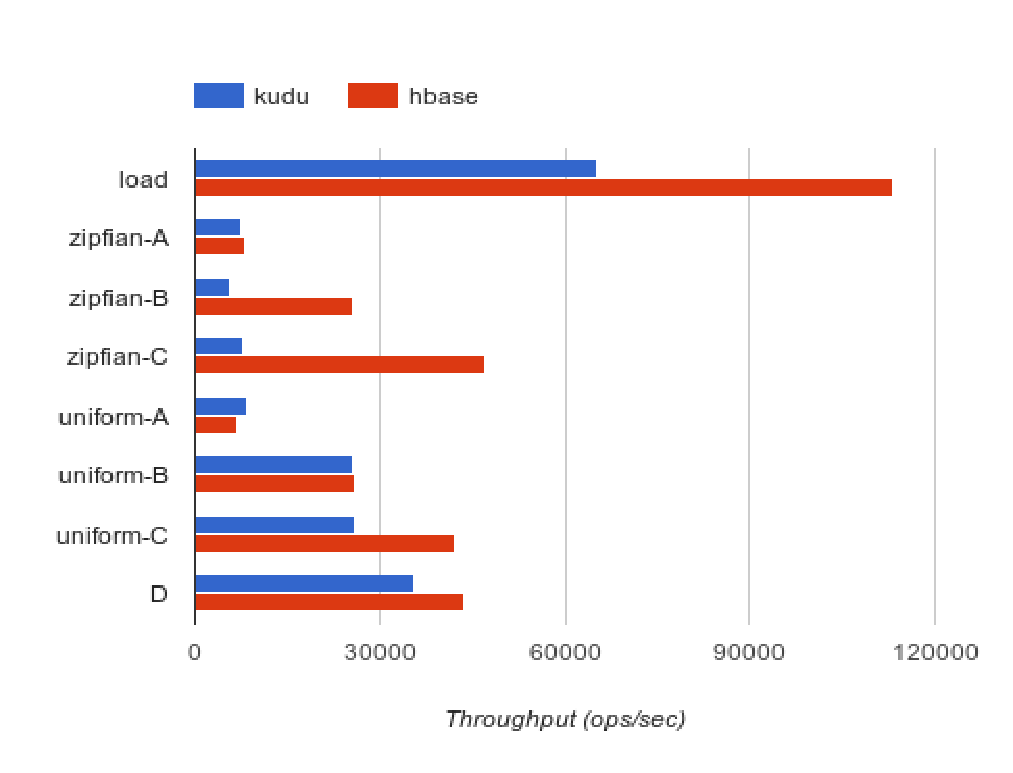
\includegraphics[width=3.5in]{ycsb-results.pdf}
  \caption{Operation throughput of YCSB random-access workloads, comparing Kudu vs.\ HBase}
  \label{fig:ycsb_throughput}
\end{figure}

Figure \ref{fig:ycsb_throughput} presents the throughput reported by YCSB for each of the
workloads. In nearly all workloads, HBase out-performs Kudu in terms of throughput. In
particular, Kudu performs poorly in the Zipfian update workloads, where the CPU time
spent in reads is dominated by applying long chains of mutations stored in delta stores
\footnote{We have identified several potential optimizations in this code path, tracked
in $KUDU-749$.}. HBase, on the other hand, has long targeted this type of online workload
and performs comparably in both access distributions.

Due to time limitations in preparing this paper for the first Kudu beta release, we do
not have sufficient data to report on longer-running workloads, or to include a summary
of latency percentiles. We anticipate updating this paper as results become available.

% \section{Conclusion}
% TODO

\section{Acknowledgements}
Kudu has benefited from many contributors outside of the authors of this paper. In particular, thanks to Chris Leroy, Binglin Chang, Guangxiang Du, Martin Grund, Eli Collins, Vladimir Feinberg, Alex Feinberg, Sarah Jelinek, Misty Stanley-Jones, Brock Noland, Michael Crutcher, Justin Erickson, and Nong Li.

\bibliographystyle{abbrv}
\bibliography{kudu}

\end{document}
